\documentclass{beamer}
\usepackage{listings,bm}
\usepackage{hyperref}
\usepackage{tikz}
\usetikzlibrary{positioning,shadows,arrows,shapes,calc}
\usepackage{tipa}
\DeclareMathOperator*{\softmax}{softmax}
\newcommand{\ipa}[1]{\fontfamily{cmr}\selectfont\textipa{#1}}
\def\labelenumi\theenumi
\usepackage{graphicx}
\usepackage{amsmath}
\mode<presentation>{\usetheme{Frankfurt}}
\AtBeginSection
{
  \begin{frame}<beamer>
    \frametitle{Outline}
    \tableofcontents[currentsection,currentsubsection]
  \end{frame}
}
\title{Lecture 21: Transformer}
\author{Mark Hasegawa-Johnson\\These slides are in the public domain}
\date{ECE 417: Multimedia Signal Processing}
\institute{University of Illinois}
\titlegraphic{\includegraphics[width=0.3in]{exp/block-I-primary.png}}
\begin{document}

% Title
\begin{frame}
  \maketitle
\end{frame}

% Title
\begin{frame}
  \tableofcontents
\end{frame}

%%%%%%%%%%%%%%%%%%%%%%%%%%%%%%%%%%%%%%%%%%%%
\section[Cauchy-Schwartz]{The Cauchy-Schwartz Inequality and Cosine Distance}
\setcounter{subsection}{1}

\begin{frame}
  \frametitle{The Cauchy-Schwartz Inequality}

  The Cauchy-Schwart inequality says that, for any two vectors
  $\bm{x}=[x_1,\ldots,x_N]^T$ and $\bm{y}=[y_1,\ldots,y_N]^T$,
  \begin{displaymath}
    \vert\bm{x}^T\bm{y}\vert \le \Vert\bm{x}\Vert \Vert\bm{y}\Vert
  \end{displaymath}
  If we define the unit vectors as follows,
  \begin{displaymath}
    \hat{\bm{x}}=\frac{\bm{x}}{\Vert\bm{x}\Vert},~~~
    \hat{\bm{y}}=\frac{\bm{y}}{\Vert\bm{y}\Vert},
  \end{displaymath}
  then the Cauchy-Schwartz inequality says that
  \begin{displaymath}
    -1 \le \hat{\bm{x}}^T\hat{\bm{y}} \le 1
  \end{displaymath}
\end{frame}

\begin{frame}
  \frametitle{The Cauchy-Schwartz Inequality: Proof}

  Suppose we have a particular $\bm{x}$, and we want to:
  \begin{itemize}
  \item choose $y_1,\ldots,y_N$ in order to maximize
    the dot product,
    \begin{displaymath}
      \bm{x}^T\bm{y}=\sum_{i=1}^N x_iy_i
    \end{displaymath}
  \item subject to the constraint that the length of $\bm{y}$ is
    fixed, say,
    \begin{displaymath}
      1 = \sum_{i=1}^N y_i^2
    \end{displaymath}
  \end{itemize}
  This can be done by choosing $y_1,\ldots,y_N$ to maximize the
  following Lagrangian:
  \begin{displaymath}
    {\mathcal L}(\bm{y}) = \sum_{i=1}^N x_iy_i + \lambda\left(\sum_{i=1}^N y_i^2-1\right)
  \end{displaymath}
\end{frame}

\begin{frame}
  \frametitle{The Cauchy-Schwartz Inequality: Proof}

  \begin{displaymath}
    {\mathcal L}(\bm{y}) = \sum_{i=1}^N x_iy_i +\lambda\left(\sum_{i=1}^N y_i^2-1\right)
  \end{displaymath}
  Setting $\frac{\partial{\mathcal L}}{\partial y_i}=0$ yields:
  \begin{displaymath}
    y_i = -\frac{x_i}{2\lambda},
  \end{displaymath}
  There are two values of $\lambda$ that satisfy the constraint
  $\Vert\bm{y}\Vert=1$.  They are:
  \begin{displaymath}
    y_i = \pm \frac{x_i}{\Vert\bm{x}\Vert}
  \end{displaymath}
\end{frame}

\begin{frame}
  \frametitle{Cosine Distance}
  \begin{columns}
    \begin{column}{0.5\textwidth}
      The Cauchy-Schwartz inequality can be written as:
      \begin{displaymath}
        -1 \le \hat{\bm{x}}^T\hat{\bm{y}}\le 1,
      \end{displaymath}
      where $\hat{\bm{x}}=\frac{\bm{x}}{\Vert\bm{x}\Vert}$ and
      $\hat{\bm{y}}=\frac{\bm{y}}{\Vert\bm{y}\Vert}$.  This is an
      $N$-dimensional generalization of the 2D geometric
      interpretation of the dot product:
      \begin{displaymath}
        \hat{\bm{x}}^T\hat{\bm{y}} = \cos\phi
      \end{displaymath}
    \end{column}
    \begin{column}{0.5\textwidth}
      \begin{center}
        \includegraphics[width=\textwidth]{exp/Cauchy-Schwarz_inequation_in_Euclidean_plane.png}

        CC-SA 4.0,
        \url{https://commons.wikimedia.org/wiki/File:Cauchy-Schwarz_inequation_in_Euclidean_plane.gif}
      \end{center}
    \end{column}
  \end{columns}
\end{frame}
        
\begin{frame}
  \frametitle{Cosine Distance}
  \begin{columns}
    \begin{column}{0.5\textwidth}
      Large-magnitude vectors have a tendency to swamp the training
      criterion for a neural net.  It's often useful to explicitly
      ignore the magnitude of the vector, and to only minimize the
      angle between two vectors on the $(N-1)$-dimensional
      hypersphere.  This is done by minimizing the {\bf cosine distance},
      \begin{align*}
        \mbox{cosd}(\bm{x},\bm{y}) &=
        1-\cos(\bm{x},\bm{y})\\
        &= 1- \hat{\bm{x}}^T\hat{\bm{y}}
      \end{align*}
      Which is equivalent to maximizing the {\bf cosine similarity},
      $\hat{\bm{x}}^T\hat{\bm{y}}$.
    \end{column}
    \begin{column}{0.5\textwidth}
      \begin{center}
        \includegraphics[width=\textwidth]{exp/Cauchy-Schwarz_inequation_in_Euclidean_plane.png}

        \begin{tiny}
          CC-SA 4.0,
          \url{https://commons.wikimedia.org/wiki/File:Cauchy-Schwarz_inequation_in_Euclidean_plane.gif}
        \end{tiny}
      \end{center}
    \end{column}
  \end{columns}
\end{frame}
        
%%%%%%%%%%%%%%%%%%%%%%%%%%%%%%%%%%%%%%%%%%%%
\section{Smart PCA}
\setcounter{subsection}{1}

\begin{frame}
  \frametitle{PCA and Smart PCA}

  Consider trying to find a set of vectors, $\bm{w}_k$ ($1\le k\le
  K$), in order to minimize
  \begin{displaymath}
    \mbox{MSE}=E\left[\Vert\bm{x}-\sum_{k=1}^Kh_k \bm{w}_k\Vert^2\right],
  \end{displaymath}
  where expectation is over the training dataset.  The minimum-MSE
  solution has orthogonal vectors, and therefore
  $h_k=\frac{\bm{w}_k^T\bm{x}}{\Vert\bm{w}_k\Vert^2}$ is the
  minimum-MSE weight.
  \begin{itemize}
  \item The MMSE solution can be computed using principal components analysis (PCA).
  \item The MMSE solution can also be computed using an autoencoder neural
    network.  If $K$ is much less than the vector dimension, the
    autoencoder computation is faster, so this is called ``smart PCA''
    (SPCA).
  \end{itemize}
\end{frame}

\begin{frame}
  \begin{columns}
    \begin{column}{0.5\textwidth}
      Consider a training database, $\{\bm{x}_1,\ldots,\bm{x}_n\}$.
      An autoencoder computes
      \begin{displaymath}
        h_{i,k} = \bm{x}_i^T \bm{w}_k,
      \end{displaymath}
      and
      \begin{displaymath}
        \bm{x}_i' = \sum_{k=1}^K h_{i,k}\bm{w}_k=\bm{W}\bm{h}
      \end{displaymath}
      then trains $\bm{W}=[\bm{w}_1,\ldots,\bm{w}_K]$ to minimize
      \begin{displaymath}
        \mbox{MSE}=\frac{1}{n}\sum_{i=1}^n \Vert\bm{x}_i-\bm{x}_i'\Vert^2
      \end{displaymath}
    \end{column}
    \begin{column}{0.5\textwidth}
      \begin{center}
        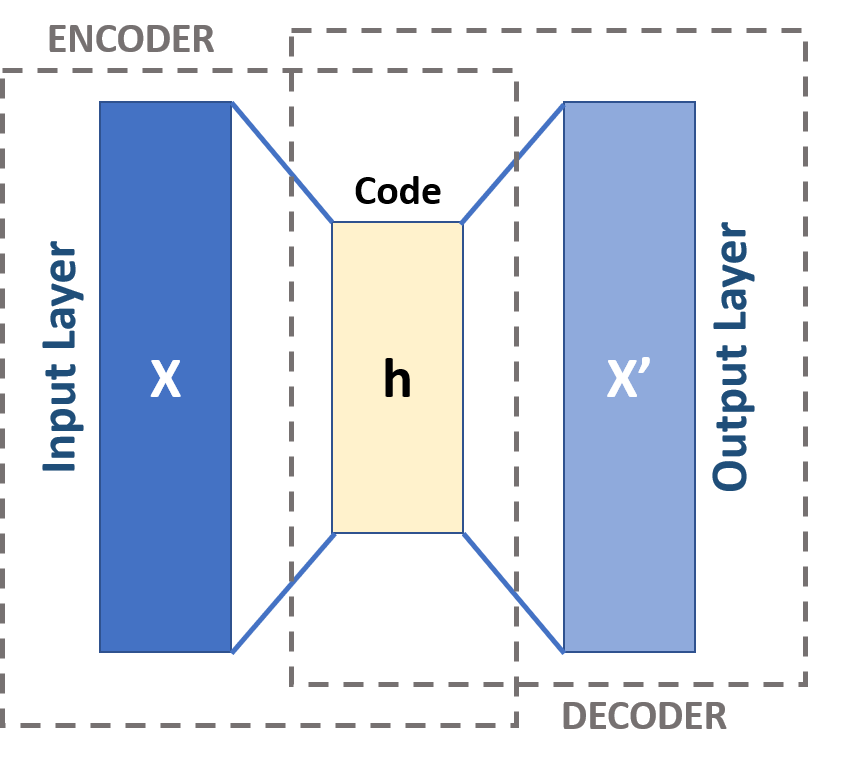
\includegraphics[width=\textwidth]{exp/Autoencoder_schema.png}

        \begin{tiny}
          CC-SA 4.0, \url{https://commons.wikimedia.org/wiki/File:Autoencoder_schema.png}
        \end{tiny}
      \end{center}
    \end{column}
  \end{columns}
\end{frame}

\begin{frame}
  \begin{columns}
    \begin{column}{0.5\textwidth}
      Both PCA and SPCA choose unit-length vectors, $\bm{W}=[\bm{w}_1,\ldots,\bm{w}_K]$ in
      order to minimize
      \begin{displaymath}
        \mbox{MSE}=E\left[\Vert\bm{x}-\bm{W}\bm{h}\Vert^2\right],
      \end{displaymath}
      therefore both SPCA and PCA choose vectors that span the same
      vector subspace.  SPCA does not decide the order of the vectors,
      or their sign, so SPCA can produce a vector subspace that's a
      rotated version of the one chosen by PCA.
    \end{column}
    \begin{column}{0.5\textwidth}
      \begin{center}
        \includegraphics[width=\textwidth]{exp/PCA_vs_Linear_Autoencoder.png}

        Plot of the first two Principal Components (left) and the two
        hidden units' values of a Linear Autoencoder (right) applied
        to the Fashion MNIST dataset. The two models being both linear
        learn to span the same subspace.
        
        \begin{tiny}
          CC-SA 4.0,
          \url{https://upload.wikimedia.org/wikipedia/commons/0/0b/PCA_vs_Linear_Autoencoder.png}
        \end{tiny}
      \end{center}
    \end{column}
  \end{columns}
\end{frame}

\begin{frame}
  \frametitle{PCA and Smart PCA}

  The training criterion for both PCA and SPCA is
  \begin{align*}
    \mbox{MSE} &=E\left[\Vert\bm{x}-\bm{W}\bm{h}\Vert^2\right]\\
    &=E\left[\Vert\bm{x}\Vert^2+\Vert\bm{W}\bm{h}\Vert^2-2\bm{x}^T\bm{W}\bm{h}\right]
  \end{align*}
  So minimizing the MSE is the same as maximizing the dot product between
  the hidden vector, $\bm{h}$, and the transformed input vector, $\bm{W}^T\bm{x}$.
  This is a kind of dot-product similarity measure.
\end{frame}

%%%%%%%%%%%%%%%%%%%%%%%%%%%%%%%%%%%%%%%%%%%%
\section{Attention}
\setcounter{subsection}{1}

\begin{frame}
  \frametitle{ASR and Machine Translation (MT): Similarities and Differences}

  The idea of an ``attention-weighted summary'' was proposed and
  refined from 2012 to 2017 in a series of papers, some of which were
  automatic speech recognition (ASR) papers, and some of which were
  neural machine translation (MT) papers.

  \begin{center}
    \begin{tabular}{|l|l|l|}\hline
      & Input, Output Lengths & Input, Output Sequence Order \\\hline\hline
      ASR & Different & Same\\\hline
      MT & Different & Different\\\hline
    \end{tabular}
  \end{center}
\end{frame}

\begin{frame}
  \frametitle{Encoder-Decoder Neural Nets}
  \begin{columns}
    \begin{column}{0.5\textwidth}
      Cho et al., ``Learning Phrase Representations using RNN
      Encoder–Decoder for Statistical Machine Translation''
      (Sep. 2014) proposed a solution:
      \begin{itemize}
      \item RNN ``encodes'' all of the input to a summary vector, $\bm{c}$, then
      \item RNN ``decodes'' $\bm{c}$ in order to produce the output.
      \end{itemize}
    \end{column}
    \begin{column}{0.5\textwidth}
      \begin{center}
        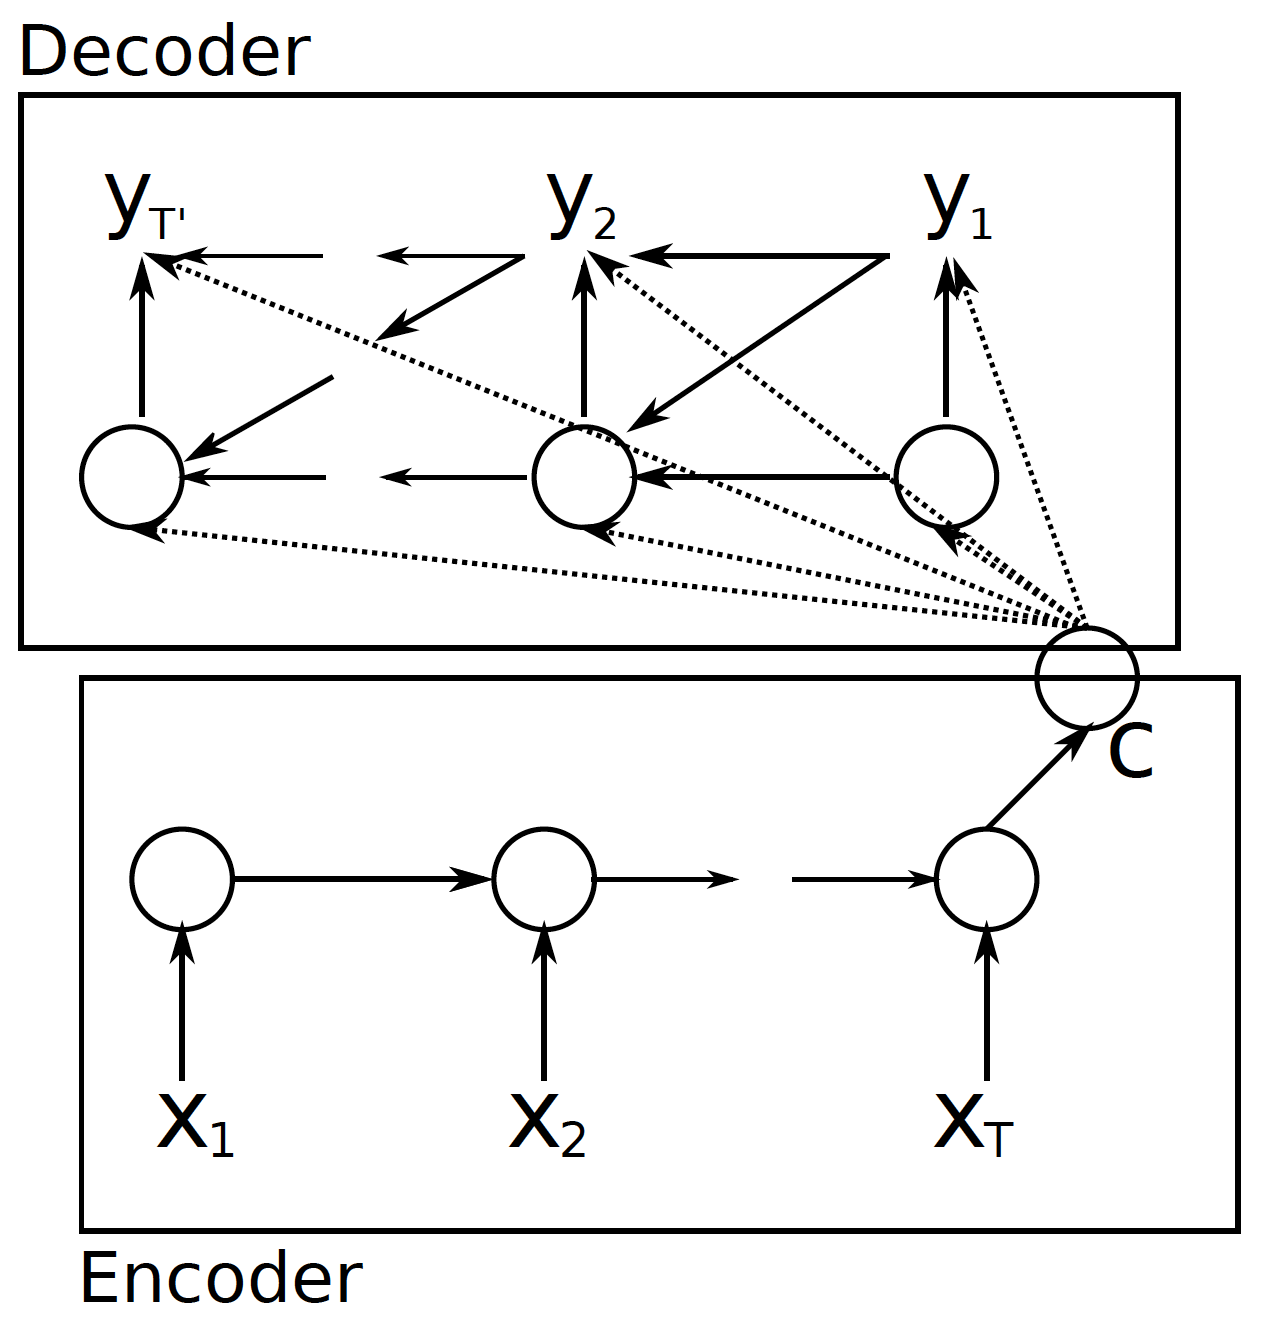
\includegraphics[width=\textwidth]{figs/cho2014sep_fig1.png}

        \begin{tiny}
          Cho, Merri{\"{e}}nboer, Gulcehre, Bahdenau, Bougares,
          Schwenk \& Bengio, Learning Phrase Representations using RNN
          Encoder–Decoder for Statistical Machine Translation, Fig.~1.
        \end{tiny}
      \end{center}
    \end{column}
  \end{columns}
\end{frame}
  
\begin{frame}
  \frametitle{Encoder-Decoder Neural Nets}
  \begin{columns}
    \begin{column}{0.4\textwidth}
      Cho et al., ``On the Properties of Neural Machine Translation:
      Encoder–Decoder Approaches'' (Oct. 2014) proposed that the
      encoder summary didn't need to be a single vector, it could be a
      sequence of vectors.
    \end{column}
    \begin{column}{0.6\textwidth}
      \begin{center}
        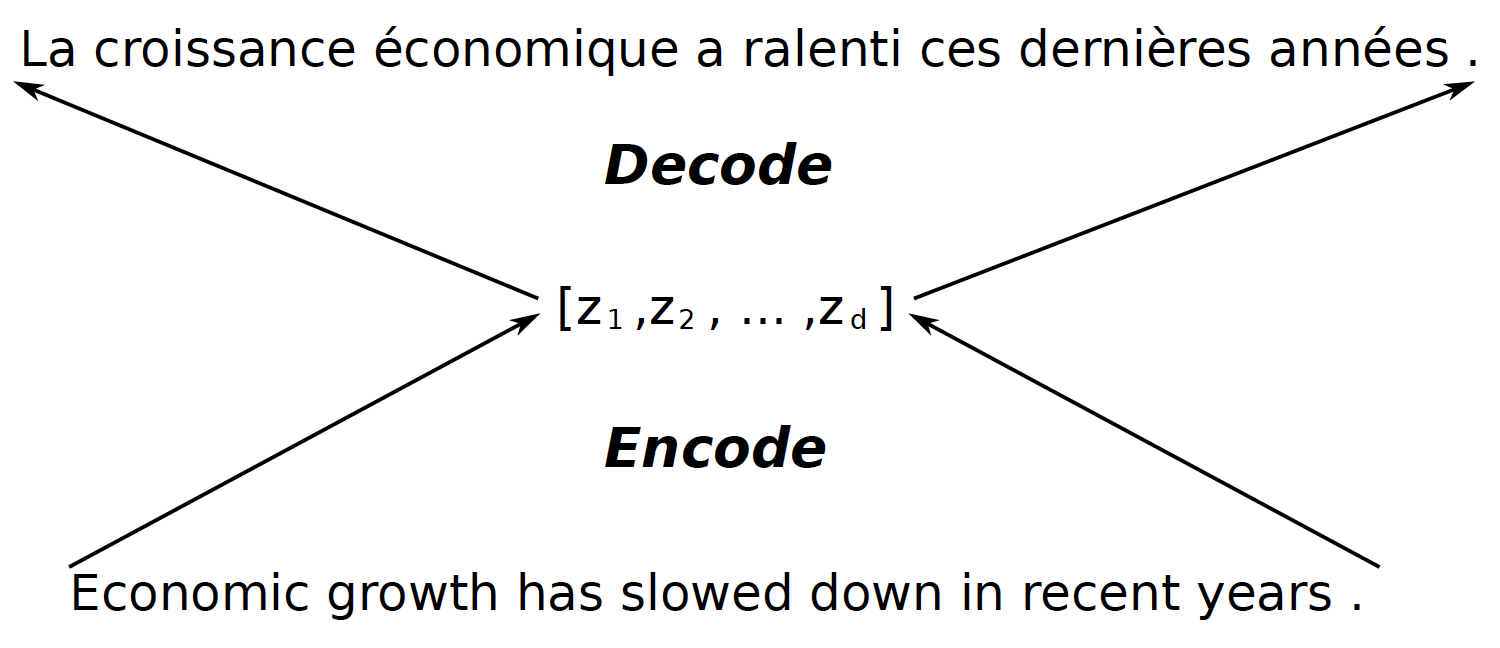
\includegraphics[width=\textwidth]{figs/cho2014oct_fig3.png}

        \begin{tiny}
          Cho, Merri{\"{e}}nboer, Bahdenau \& Bengio, On the
          Properties of Neural Machine Translation: Encoder–Decoder
          Approaches, Fig.~3.
        \end{tiny}
      \end{center}
    \end{column}
  \end{columns}
\end{frame}
  
\begin{frame}
  \frametitle{Encoder-Decoder: Too Much Information?}

  \begin{itemize}
  \item Encoder-decoder models beat the state of the art in some tasks
    (usually tasks with a lot of data), but had a fatal flaw.
  \item If the encoder creates a small summary, then
    it accidentally throws away important information, because it doesn't always
    know which information is important.
  \item If the encoder creates a large summary, then the decoder
    doesn't know which data to use for any given computation, so
    training takes longer, and sometimes fails.
  \end{itemize}
\end{frame}

\begin{frame}
  \frametitle{Attention}

  In December 2014, Chorowski et al. proposed a new type of
  encoder-decoder algorithm, based on ``attention.''
  \begin{itemize}
  \item The $i^{\textrm{th}}$ time step in the {\bf Decoder} is
    computed based on an attention-weighted summary of the inputs:
    \begin{displaymath}
      \bm{s}_i = \mbox{Recurrency}\left(\bm{s}_{i-1},\sum_{j=1}^L\alpha_{i,j}\bm{h}_j\right)
    \end{displaymath}
  \item The {\bf Attention} is a kind of probability mass (sums to one) over
    the different input time steps, $1\le j\le L$:
    \begin{displaymath}
      \alpha_{i,j} = \frac{\exp(e_{i,j})}{\sum_{j=1}^L \exp(e_{i,j})},~~~\sum_{j=1}^L \alpha_{i,j}=1
    \end{displaymath}
  \item The {\bf Attention Score} is a special neural net that
    measures the similarity between input vector $h_j$ and output
    vector $s_{i-1}$:
    \begin{displaymath}
      e_{i,j} = \mbox{Score}(\bm{s}_{i-1},\bm{h}_j)
    \end{displaymath}
  \end{itemize}
\end{frame}

\begin{frame}
  \frametitle{Attention}
  \begin{columns}
    \begin{column}{0.3\textwidth}
      \begin{itemize}
      \item $\bm{s}_{i-1}$ and $\bm{h}_j$ determine $\alpha_{i,j}$
      \item $\bm{s}_i$ is determined by $\sum_{j=1}^L \alpha_{i,j}\bm{h}_j$
      \end{itemize}
    \end{column}
    \begin{column}{0.7\textwidth}
      \begin{center}
        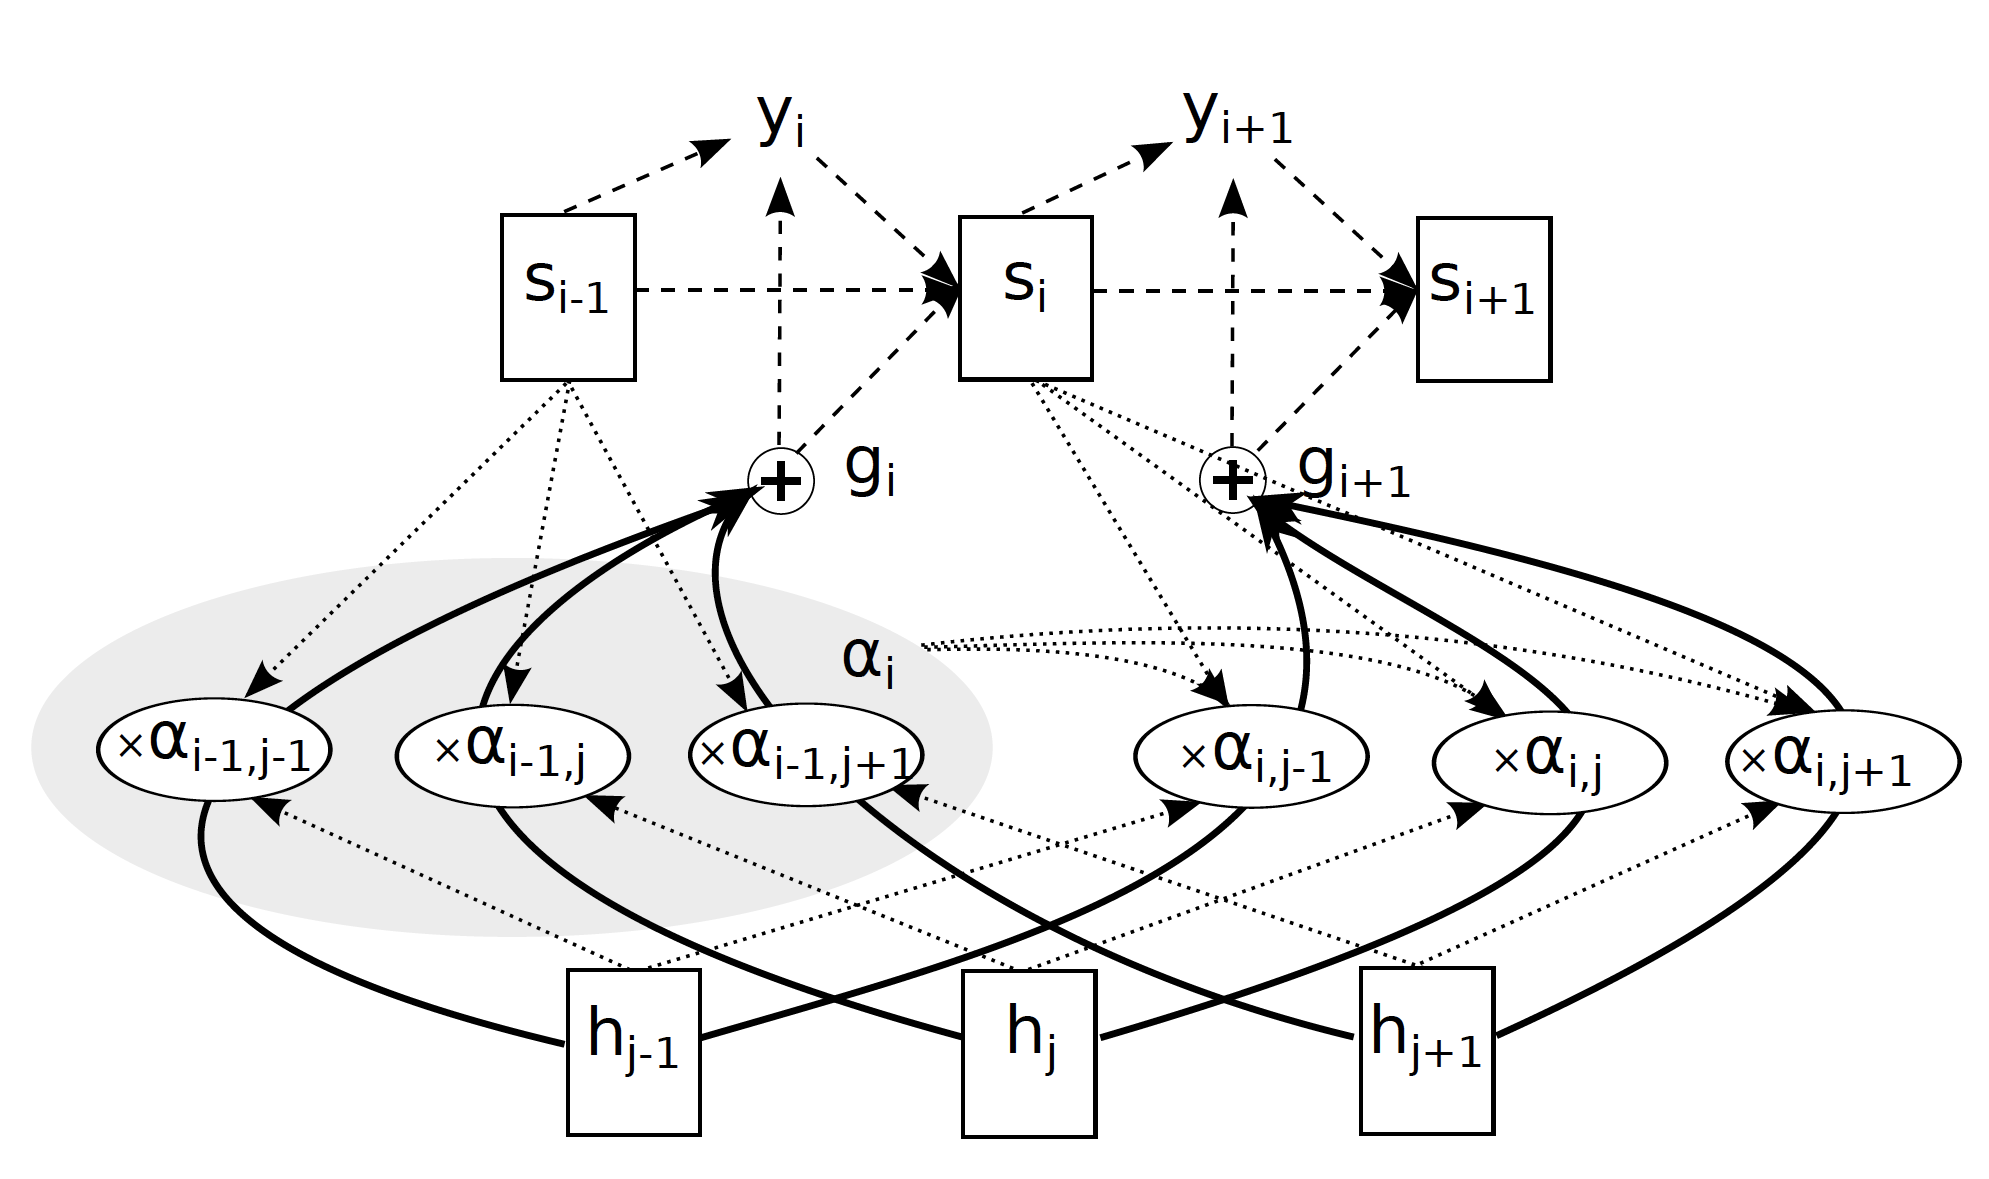
\includegraphics[width=\textwidth]{figs/chorowski2014fig1.png}

        \begin{tiny}
          Chorowski, Bahdanau, Serdyk, Cho \& Bengio, Attention-Based
          Models for Speech Recognition, Fig. 1
        \end{tiny}
      \end{center}
    \end{column}
  \end{columns}
\end{frame}

\begin{frame}
  \frametitle{When should you pay attention?}

  \begin{itemize}
    \item 
      The key idea of attention is that there is some sort of similarity
      score, $e_{i,j}=\mbox{Similarity}(\bm{s}_{i-1},\bm{h}_j)$, so that you can
      compute attention weights according to
      \begin{displaymath}
        \alpha_{i,j} = \frac{\exp(e_{i,j})}{\sum_{j=1}^L \exp(e_{i,j})}
      \end{displaymath}
    \item
      Raw inputs (speech) and raw outputs (text) are not inherently
      similar.
    \item
      There needs to be a network that converts the inputs into
      some hidden vectors, $\bm{h}_j$ and $\bm{s}_{i-1}$, that are similar if
      and only if $\alpha_{i,j}$ should be large.
  \end{itemize}
\end{frame}


\begin{frame}
  \begin{columns}
    \begin{column}{0.4\textwidth}
      Cheng, Dong and Lapata, ``Long Short-Term Memory-Networks for
      Machine Reading,'' proposed using a new kind of attention called
      ``intra-attention'' or ``self-attention'' to compute
      \begin{itemize}
      \item $\bm{h}_j$ from the inputs, and
      \item $\bm{s}_{i-1}$ from the preceding outputs, so that
      \item inter-attention will correctly measure
        $\mbox{Similarity}(\bm{s}_{i-1},\bm{h}_j)$.
      \end{itemize}
    \end{column}
    \begin{column}{0.6\textwidth}
      \begin{center}
        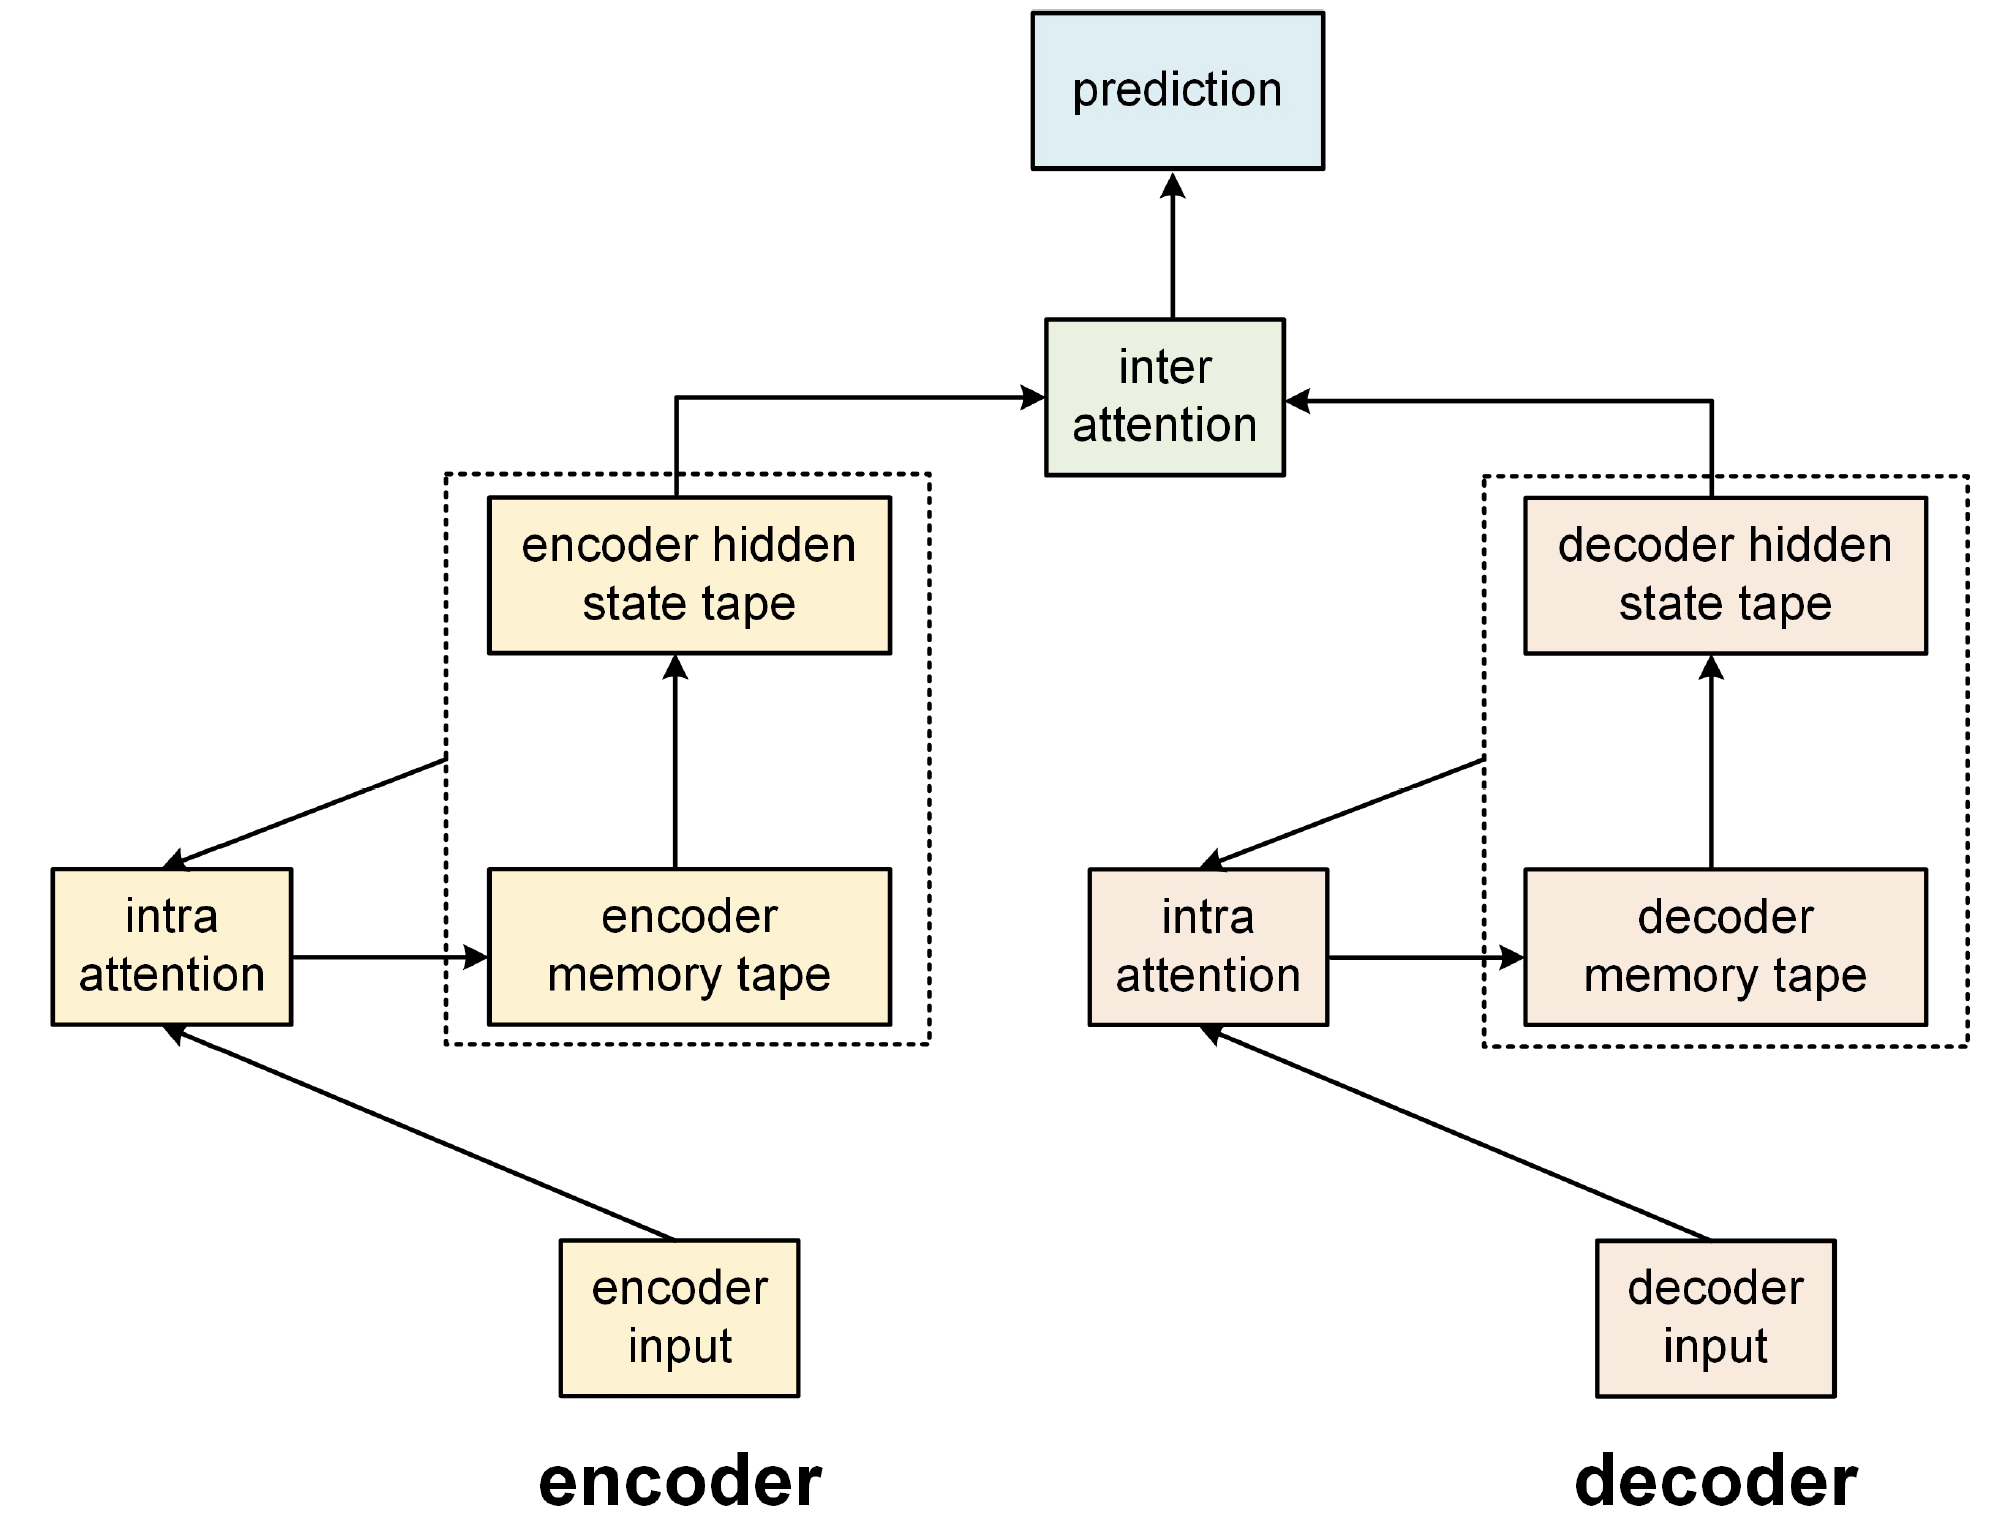
\includegraphics[width=\textwidth]{figs/cheng2016fig3a.png}

        \begin{tiny}
          Cheng, Dong \& Lapata, ``Long Short-Term Memory-Networks for
          Machine Reading,'' 2016, Fig. 3(a)
        \end{tiny}
      \end{center}
    \end{column}
  \end{columns}
\end{frame}


\begin{frame}
  \frametitle{Intra-Attention}

  An RNN with intra-attention computes the RNN state vector
  $\tilde{h}_t$ as the attention-weighted summary of past RNN state
  vectors:
  \begin{displaymath}
    \tilde{\bm{h}}_t = \sum_{i=1}^{t-1} \alpha_{t,i} \bm{h}_i,
  \end{displaymath}
  where the weights, $\alpha_{t,i}$, are softmax normalized:
  \begin{displaymath}
    \alpha_{t,i} = \softmax(e_{t,i}),
  \end{displaymath}
  based on similarities computed between $\bm{h}_i$, $\tilde{\bm{h}}_{t-1}$, and
  the input vector $\bm{x}_t$:
  \begin{displaymath}
    e_{t,i} = \bm{w}_e^T\tanh\left(\bm{W}_h\bm{h}_i+\bm{W}_x\bm{x}_t+\bm{W}_{\tilde{h}}\tilde{\bm{h}}_{t-1}\right)
  \end{displaymath}
\end{frame}

\begin{frame}
  \begin{columns}
    \begin{column}{0.4\textwidth}
      \begin{itemize}
        \item 
          The representation of each word (in red) is
          computed based on\ldots
        \item
          an attention-weighted summary of all previous
          words (attention weights in blue).
        \item
          Thus, the meaning of a word depends on its context.
      \end{itemize}
    \end{column}
    \begin{column}{0.6\textwidth}
      \begin{center}
        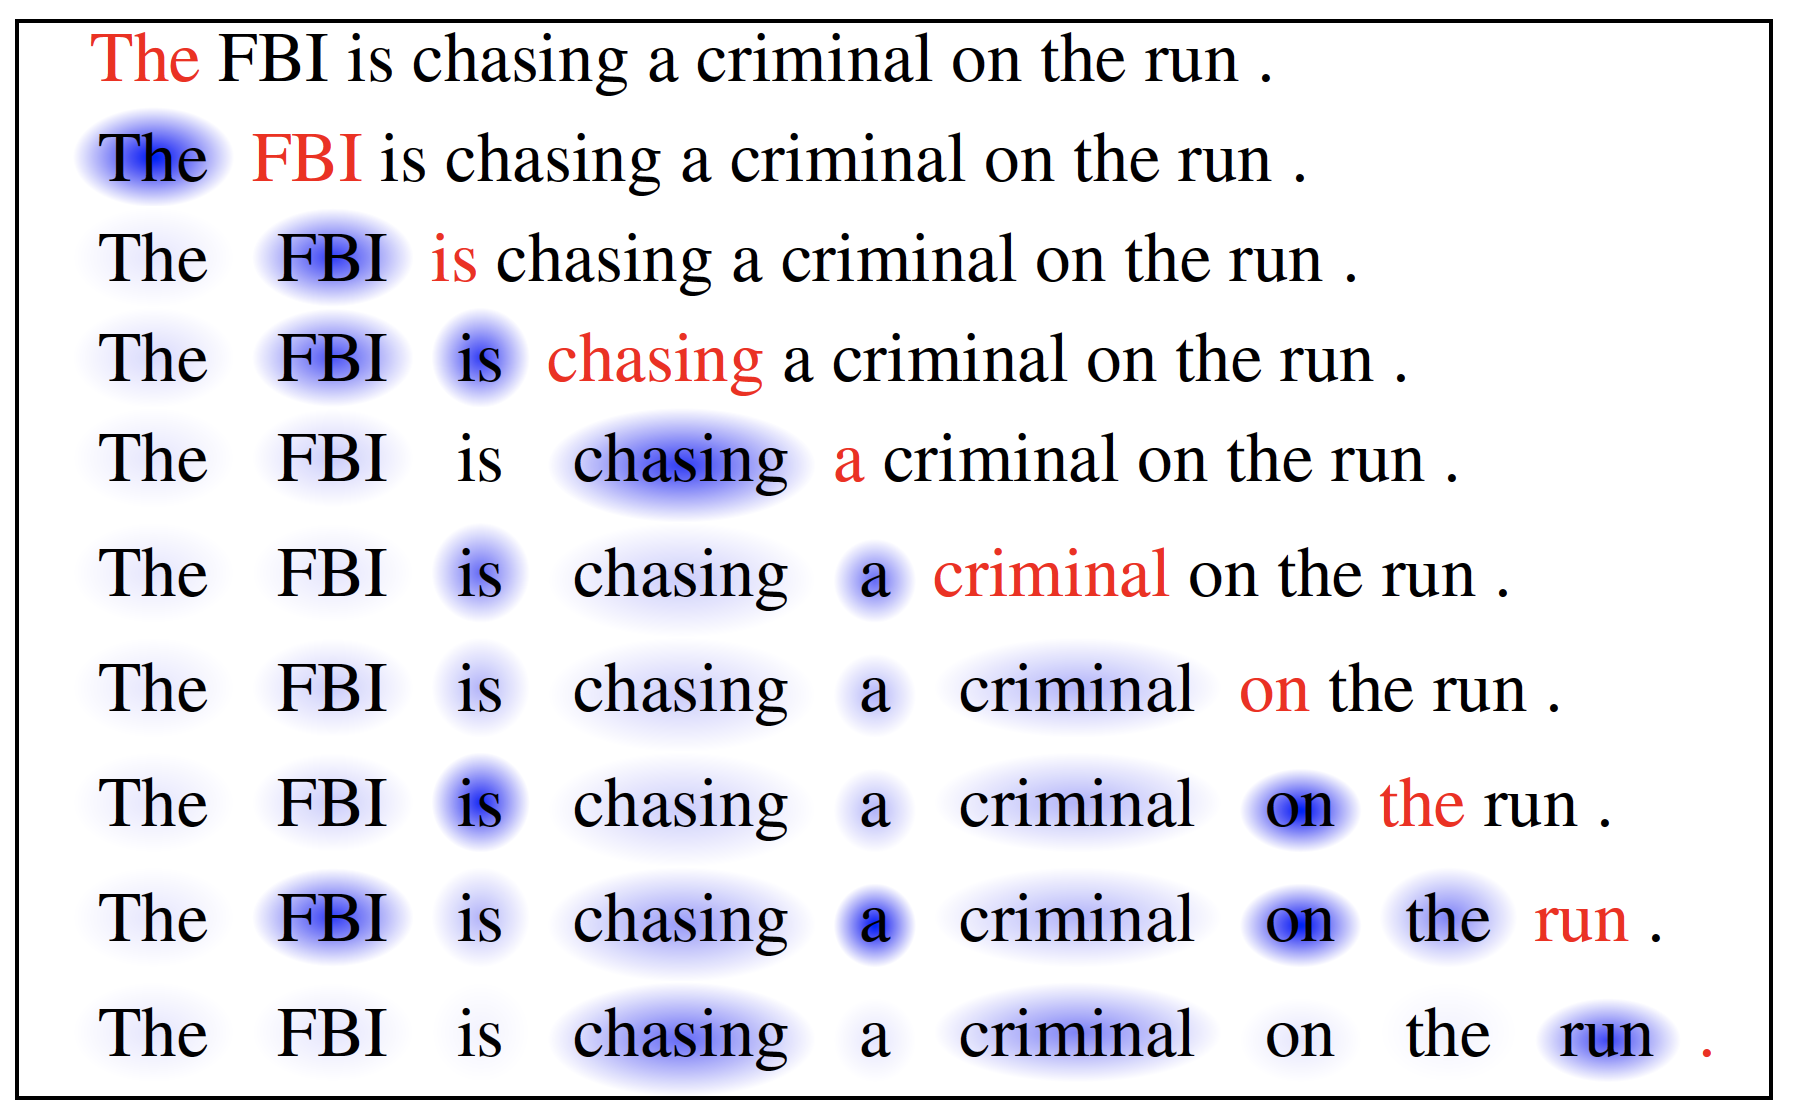
\includegraphics[width=\textwidth]{figs/cheng2016fig1.png}

        \begin{tiny}
          Cheng, Dong \& Lapata, ``Long Short-Term Memory-Networks for
          Machine Reading,'' 2016, Fig. 1
        \end{tiny}
      \end{center}
    \end{column}
  \end{columns}
\end{frame}


%%%%%%%%%%%%%%%%%%%%%%%%%%%%%%%%%%%%%%%%%%%%
\section{Transformer}
\setcounter{subsection}{1}

\begin{frame}
  \frametitle{Transformer: Scaled Transformed Dot-Product Attention}

  \begin{center}
    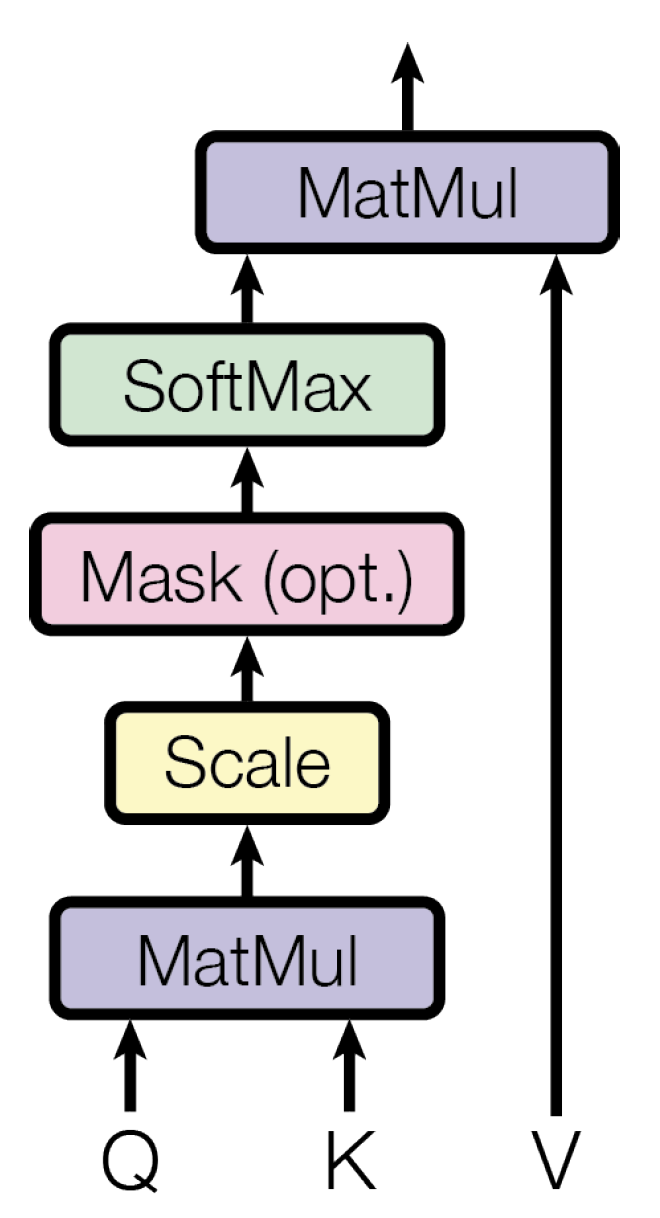
\includegraphics[height=0.8\textheight]{figs/vaswani2017fig2a.png}

    \begin{tiny}
      Vaswani et al., 2017, Figure 2(a)
    \end{tiny}
  \end{center}
\end{frame}

\begin{frame}
  \frametitle{The Data Matrices}

  \begin{displaymath}
    \bm{Q} = \left[\begin{array}{c}\bm{q}_1^T\\\vdots\\\bm{q}_n^T\end{array}\right],~~~
    \bm{K} = \left[\begin{array}{c}\bm{k}_1^T\\\vdots\\\bm{k}_n^T\end{array}\right],~~~
    \bm{V} = \left[\begin{array}{c}\bm{v}_1^T\\\vdots\\\bm{v}_n^T\end{array}\right]
  \end{displaymath}
  \begin{itemize}
  \item $\bm{q}_i\in\Re^{d_k}$ is a query vector
  \item $\bm{k}_j\in\Re^{d_k}$ is a key vector
  \item $\bm{v}_j\in\Re^{d_v}$ is a value vector
  \end{itemize}
\end{frame}

\begin{frame}
  \frametitle{The Dot-Product}

  \begin{align*}
    \bm{Q}\bm{K}^T &=
    \left[\begin{array}{ccc}
        \bm{q}_1^T\bm{k}_1 & \cdots & \bm{q}_1^T\bm{k}_n\\
        \vdots & \ddots & \vdots \\
        \bm{q}_n^T\bm{k}_1 & \cdots & \bm{q}_n^T\bm{k}_n
      \end{array}\right],
  \end{align*}
  is the matrix whose $(i,j)^{\textrm{th}}$ element is the dot product between $\bm{q}_i$ and $\bm{k}_j$.
\end{frame}

\begin{frame}
  \frametitle{The Scaled Dot-Product}
  
  Suppose that $\bm{q}_i$ and $\bm{k}_j$ are each normalized so that they are
  independent Gaussian random variables with zero mean and unit variance.  Then
  \begin{displaymath}
    \bm{q}_i^T\bm{k}_j = \sum_{t=1}^{d_k} q_{i,t}k_{j,t}
  \end{displaymath}
  is a zero-mean random variable with variance $d_k$.  We can
  re-normalize it (to zero mean and unit variance) by computing
  \begin{displaymath}
    \frac{\bm{q}_i^T\bm{k}_j}{\sqrt{d_k}} = \frac{1}{\sqrt{d_k}}\sum_{t=1}^{d_k} q_{i,t}k_{j,t}
  \end{displaymath}
\end{frame}

\begin{frame}
  \frametitle{Scaled Dot-Product Attention}

  We assume that $\bm{q}_i$ and $\bm{k}_j$ have been transformed by
  some preceding neural net, so $\bm{q}_i^T\bm{k}_j$ is large if and
  only if they should be considered similar.  Therefore the similarity
  score is
  \begin{displaymath}
    e_{i,j} = \frac{1}{\sqrt{d_k}} \bm{q}_i^T\bm{k}_j,
  \end{displaymath}
  and the corresponding attention weight is
  \begin{displaymath}
    \alpha_{i,j} = \softmax(e_{i,j}) = \frac{\exp(e_{i,j})}{\sum_{j=1}^n \exp(e_{i,j})}
  \end{displaymath}
  \begin{displaymath}
    \left[\begin{array}{ccc}
        \alpha_{1,1}&\cdots&\alpha_{1,n}\\
        \vdots&\ddots&\vdots\\
        \alpha_{n,1}&\cdots&\alpha_{n,n}
      \end{array}\right]
    = \softmax\left(\frac{\bm{Q}\bm{K}^T}{\sqrt{d_k}}\right)
  \end{displaymath}
\end{frame}

\begin{frame}
  \frametitle{Scaled Dot-Product Attention}

  The context summary vector is then
  \begin{displaymath}
    \bm{c}(\bm{q}_i) = \sum_{j=1}^n \alpha_{i,j} \bm{v}_j
  \end{displaymath}
  If we stack these up into a matrix, we get
  \begin{displaymath}
    \left[\begin{array}{c}\bm{c}(\bm{q}_1)^T\\\vdots\\\bm{c}(\bm{q}_n)^T\end{array}\right] =
    \softmax\left(\frac{\bm{Q}\bm{K}^T}{\sqrt{d_k}}\right)
    \left[\begin{array}{c}\bm{v}_1^T\\\vdots\\\bm{v}_n^T\end{array}\right]
  \end{displaymath}
\end{frame}

\begin{frame}
  \frametitle{Masking}

  If $\bm{q}_i$, $\bm{k}_j$ and $\bm{v}_j$ are decoder vectors being
  produced autoregressively (e.g., decoder self-attention), then
  $\bm{c}(\bm{q}_i)$ can only depend on values of $\bm{v}_j$ for
  $j<i$:
  \begin{displaymath}
    \bm{c}(\bm{q}_i) = \sum_{j=1}^{i-1} \alpha_{i,j} \bm{v}_j
  \end{displaymath}
  This can be done by setting $\alpha_{i,j}=0$ for $j\ge i$.  In turn,
  this can be done by masking the similarity scores as follows:
  \begin{displaymath}
    e_{i,j} = \frac{1}{\sqrt{d_k}} \bm{q}_i^T\bm{k}_j + m_{i,j},
  \end{displaymath}
  where
  \begin{displaymath}
    m_{i,j} = \left\{\begin{array}{ll}
    0 & j < i\\
    -\infty & j\ge i
    \end{array}\right.
  \end{displaymath}
\end{frame}

\begin{frame}
  \frametitle{Scaled Dot-Product Attention}

  \begin{columns}
    \begin{column}{0.5\textwidth}
      \begin{align*}
        &\text{Attention}(\bm{Q},\bm{K},\bm{V}) \\
        &=
        \softmax\left(\frac{\bm{Q}\bm{K}^T}{\sqrt{d_k}}\right)\bm{V}
      \end{align*}
    \end{column}
    \begin{column}{0.5\textwidth}
      \begin{center}
        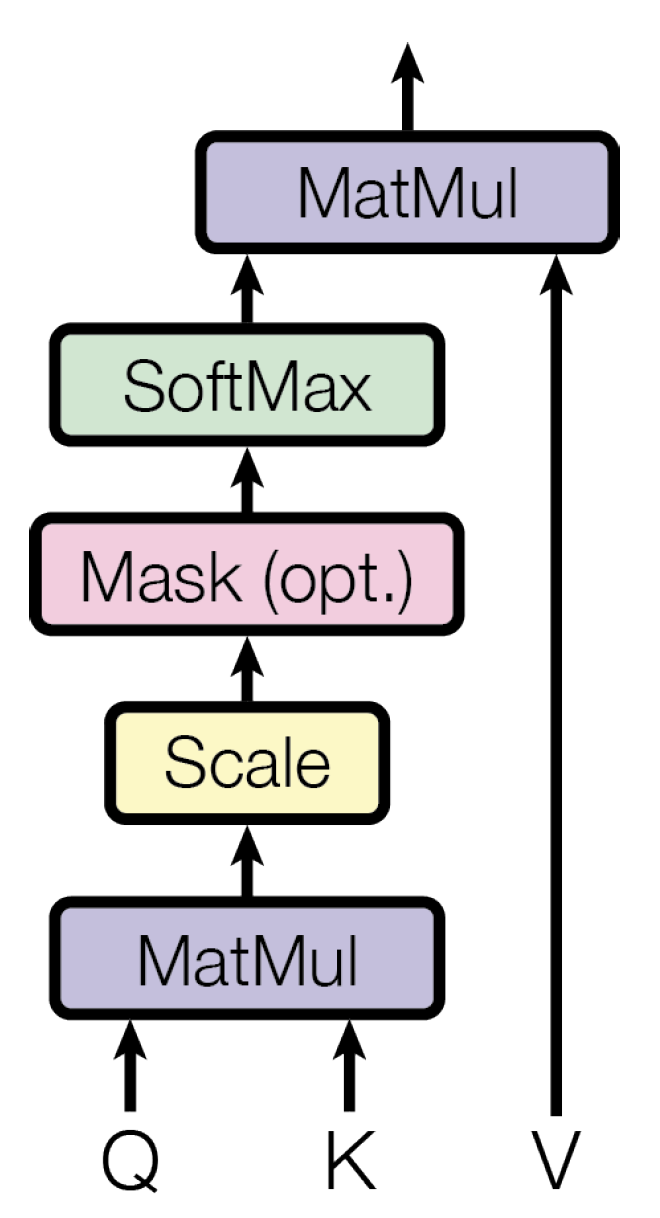
\includegraphics[height=0.8\textheight]{figs/vaswani2017fig2a.png}
        
        \begin{tiny}
          Vaswani et al., 2017, Figure 2(a)
        \end{tiny}
      \end{center}
    \end{column}
  \end{columns}
\end{frame}



%%%%%%%%%%%%%%%%%%%%%%%%%%%%%%%%%%%%%%%%%%%%
\section{Multi-Head Attention}
\setcounter{subsection}{1}

\begin{frame}
  \frametitle{Multi-Head Attention: Why}

  \begin{itemize}
  \item
    Dot-product attention assumes that $\bm{q}_i$ and $\bm{k}_j$ have already
    been transformed by some neural network so that $\bm{q}_i^T\bm{k}_{j}$ is
    large if and only if $\bm{v}_j$ is an important part of the context.
  \item
    What if you need several types of context?  One type tells you
    about speaker ID, one type tells you about dialect, one type tells
    you the topic of conversation, etc.
  \item
    Multi-Head Attention computes many different types of $\bm{q}_i$ vectors,
    and many different types of $\bm{k}_j$ vectors, so that different types
    of context may be accumulated in parallel.
  \end{itemize}
\end{frame}

\begin{frame}
  \frametitle{Multi-Head Attention}

  \begin{center}
    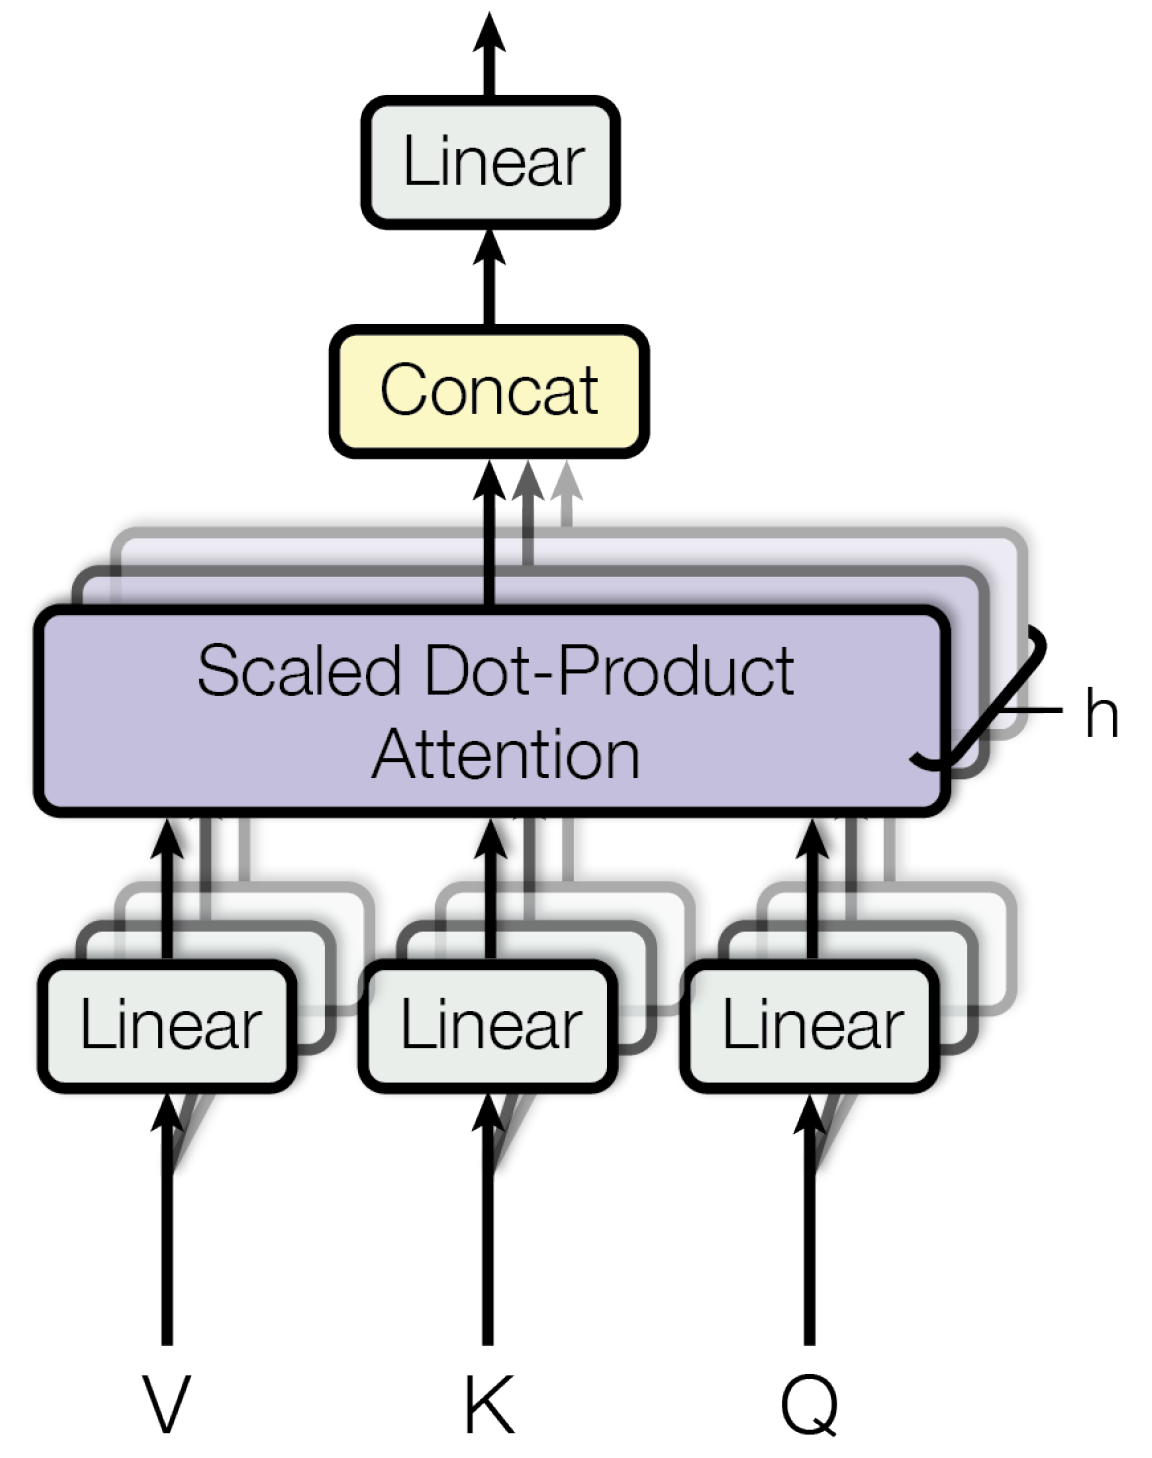
\includegraphics[height=0.8\textheight]{figs/vaswani2017fig2b.png}

    \begin{tiny}
      Vaswani et al., 2017, Figure 2(b)
    \end{tiny}
  \end{center}
\end{frame}


\begin{frame}
  \frametitle{Multi-Head Attention}

  \begin{align*}
    \text{head}_i &=
    \text{Attention}\left(\bm{Q}\bm{W}_i^Q,\bm{K}\bm{W}_i^K,\bm{V}\bm{W}_i^V\right)\\
    &=
    \softmax\left(\frac{\bm{Q}\bm{W}_i^Q(\bm{K}\bm{W}_i^{K})^T}{\sqrt{d_k}}\right)\bm{V}\bm{W}_i^V,
  \end{align*}
  where the weight matrices $\bm{W}_i^Q$, $\bm{W}_i^K$, and
  $\bm{W}_i^V$, for $1\le~i\le~h$, are learned matrices summarizing
  the type of context accumulated in each head.  Then
  \begin{displaymath}
    \text{MultiHead}(\bm{Q},\bm{K},\bm{V}) = \text{Concat}(\text{head}_1,\ldots,\text{head}_h)\bm{W}^O,
  \end{displaymath}
  where $\bm{W}^O$ is a final transformation that can, e.g., combine
  information from different heads in a learned manner.
\end{frame}

%%%%%%%%%%%%%%%%%%%%%%%%%%%%%%%%%%%%%%%%%%%%
\section[Conclusion]{Conclusions}
\setcounter{subsection}{1}

\begin{frame}
  \frametitle{Why Self-Attention?}

  \begin{itemize}
    \item 
      Encoder-decoder attention is well-established, but the
      transformations that compute $\bm{q}_i$ and $\bm{k}_j$ can be (1) convolutional,
      (2) recurrent, or (3) self-attention.  When is self-attention the
      best approach?
    \item
      Recurrent networks have to propagate information from the start
      of the sequence to the end (path length=$n$).  Information can
      get forgotten.
    \item
      Convolutional networks are much quicker, but need to learn
      weights covering the entire width of the kernel ($k$).  For
      reasons of data-efficient learning, most systems therefore use
      small $k$.
    \item
      Self-attention is as fast as convolution, without pre-trained
      kernel weights.  Instead, the attention weights are based on
      similarity, which is computed using a more efficient network.
      Therefore, the ``kernel width'' for self-attention is usually
      $k=n$.
  \end{itemize}
\end{frame}


\begin{frame}
  \frametitle{Why Self-Attention?}

  \begin{center}
    \begin{tabular}{lcc}\hline
      Layer Type & Complexity/Layer & Path Length \\\hline
      Recurrent & $O\{nd^2\}$ & $O\{n\}$ \\ 
      Convolutional & $O\{knd^2\}$ & $O\{\log_k(n)\}$ \\ 
      Self-Attention & $O\{n^2d\}$ & $O\{1\}$ \\\hline
    \end{tabular}
  \end{center}
  \begin{itemize}
  \item $n=$ sequence length
  \item $d=$ representation dimension
  \item $k=$ kernel dimension
  \end{itemize}
\end{frame}

\begin{frame}
  \begin{columns}
    \begin{column}{0.5\textwidth}
      \begin{itemize}
      \item Because of the shorter pathlength, Transformer trains
        faster than LSTM.
      \item Transformer sometimes overtrains (time alignment is too
        flexible).
      \item Overtraining can be compensated by data augmentation,
        giving it exactly the same accuracy as LSTM.
      \end{itemize}
    \end{column}
    \begin{column}{0.5\textwidth}
      \begin{center}
        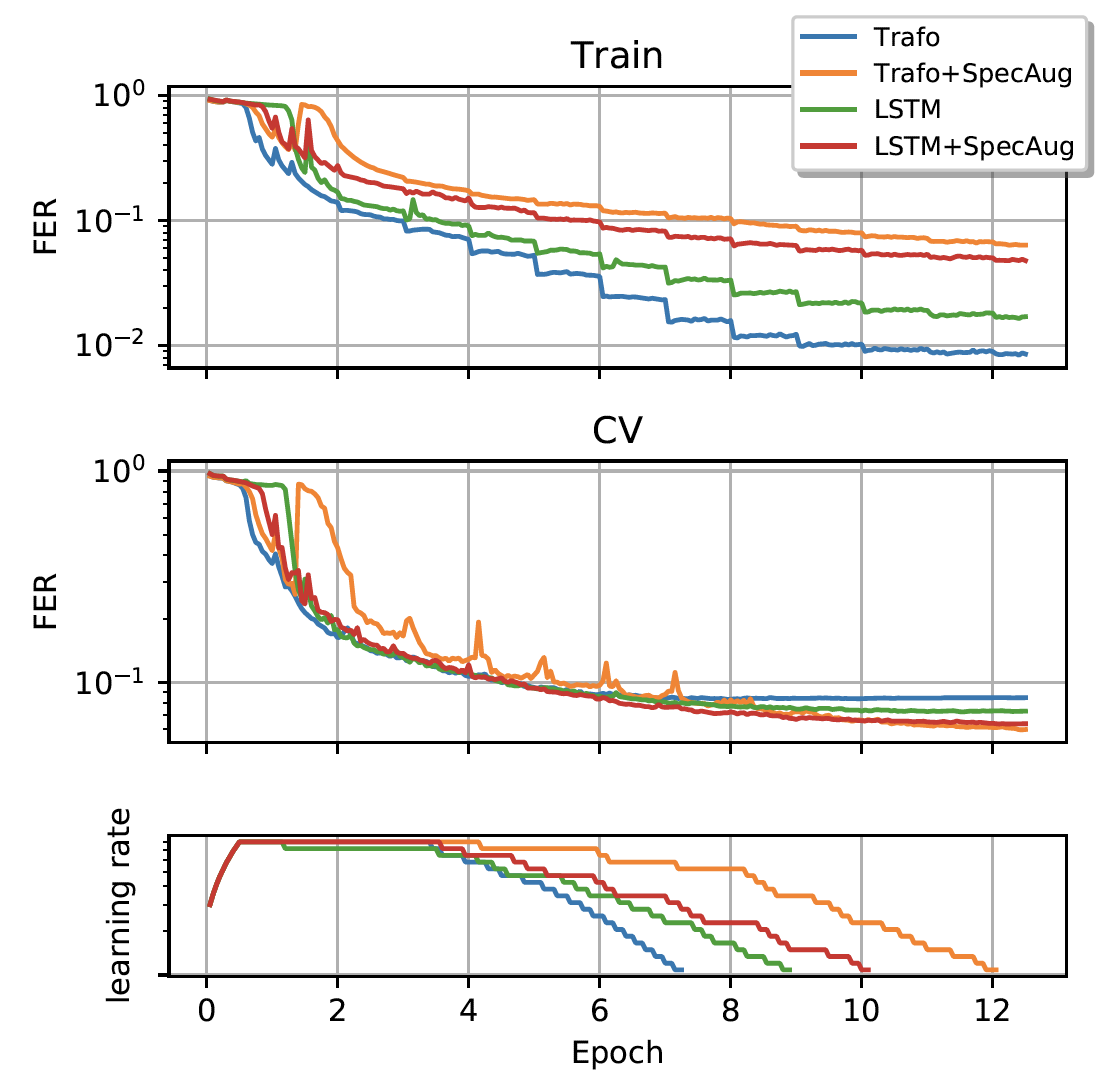
\includegraphics[width=\textwidth]{figs/zeyer2019fig1.png}

        \begin{tiny}
          Zeyer et al., ``A Comparison of Transformer and LSTM Encoder Decoder Models for ASR,''
          (c) IEEE, 2019
        \end{tiny}
      \end{center}
    \end{column}
  \end{columns}
\end{frame}

\begin{frame}
  \frametitle{Summary}

  \begin{displaymath}
    \text{Attention}(\bm{Q},\bm{K},\bm{V}) =
    \softmax\left(\frac{\bm{Q}\bm{K}^T}{\sqrt{d_k}}\right)\bm{V}
  \end{displaymath}
  \begin{displaymath}
    \text{head}_i =
    \text{Attention}\left(\bm{Q}\bm{W}_i^Q,\bm{K}\bm{W}_i^K,\bm{V}\bm{W}_i^V\right)
  \end{displaymath}
  \begin{displaymath}
    \text{MultiHead}(\bm{Q},\bm{K},\bm{V}) = \text{Concat}(\text{head}_1,\ldots,\text{head}_h)\bm{W}^O,
  \end{displaymath}

\end{frame}

\end{document}

